\documentclass{standalone}
\usepackage{tikz}
%\usepackage{graphicx}
%\usetikzlibrary{decorations.pathreplacing,angles,quotes}


\begin{document}
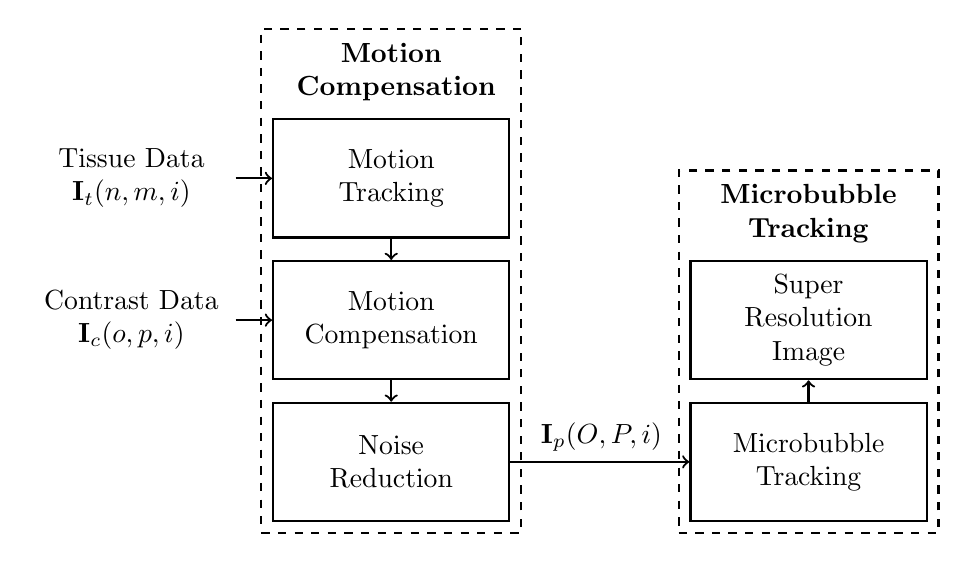
\begin{tikzpicture}
    % grid size
    \def \gs {10}
    
    \node (c1) at (0,0) [draw,thick,minimum width=3cm, text width=2.4cm, minimum height=1.5cm, align=center] {Motion\\Tracking};
    \node (c2) at (0,-1.8) [draw,thick,minimum width=3cm, text width=2.4cm, minimum height=1.5cm, align=center] {Motion\\Compensation};
    \node (c3) at (0,-3.6) [draw,thick,minimum width=3cm, text width=2.4cm, minimum height=1.5cm, align=center] {Noise\\Reduction\\};
    
    \node (l1) at (-3.3,0) [text width=2.4cm, minimum height=1.5cm, align=center] {Tissue Data $\textbf{I}_t(n,m,i)$};
    \node (l2) at (-3.3,-1.8) [text width=2.4cm, minimum height=1.5cm, align=center] {Contrast Data\\$\textbf{I}_{c}(o,p,i)$};
    
    \node (r2) at (5.3,-1.8) [draw,thick,minimum width=3cm, text width=2.4cm, minimum height=1.5cm, align=center] {Super\\Resolution\\Image};
    \node (r3) at (5.3,-3.6) [draw,thick,minimum width=3cm, text width=2.4cm, minimum height=1.5cm, align=center] {Microbubble Tracking};


    \draw [->, thick] (l1) edge (c1);
    \draw [->, thick] (l2) edge (c2);
    \draw [->, thick] (c1) edge (c2);
    \draw [->, thick] (c2) edge (c3);
    \draw [->, thick] (c3) edge (r3) node[above, xshift = 2.67cm] {$\textbf{I}_{p}(O,P,i)$};
    \draw [->, thick] (r3) edge (r2);
    
    \node (t1) at (0,-1.3) [draw,dashed,thick,minimum width=3.3cm, minimum height=6.4cm, align=center]{};
     \node[below, yshift=-2, text width=2.4cm, align=center] at (t1.north) {\textbf{Motion\\Compensation}};
    
    \node (t2) at (5.3,-2.2) [draw,dashed,thick,minimum width=3.3cm, minimum height=4.6cm, align=center]{};
    \node[below, yshift=-2, text width=2.4cm, align=center] at (t2.north) {\textbf{Microbubble\\Tracking}};
    
\end{tikzpicture}
\end{document}



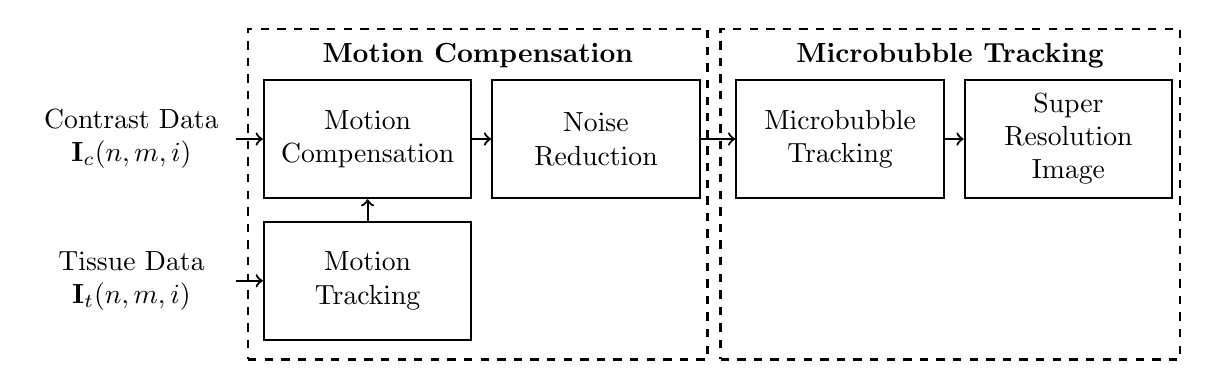
\begin{tikzpicture}
    % grid size
    \def \gs {10}

    %\draw[thick,dashed] (-0.1,0.1) rectangle (1.6,-1.1);
    \node (b1) at (-0.1,0) [text width=2.4cm, minimum height=1.5cm, align=center] {Contrast Data\\$\textbf{I}_{c}(n,m,i)$};
    \node (b2) at (2.9,-0) [draw,thick,text width=2.4cm, minimum height=1.5cm, align=center] {Motion\\Compensation};
    \node (b3) at (5.8,-0) [draw,thick,text width=2.4cm, minimum height=1.5cm, align=center] {Noise\\Reduction\\};
    \node (b4) at (8.9,-0) [draw,thick,text width=2.4cm, minimum height=1.5cm, align=center] {Microbubble Tracking};
    \node (b5) at (11.8,-0) [draw,thick,text width=2.4cm, minimum height=1.5cm, align=center] {Super\\Resolution\\Image};
    
    \node (b6) at (-0.1,-1.8) [text width=2.4cm, minimum height=1.5cm, align=center] {Tissue Data $\textbf{I}_t(n,m,i)$};
    \node (b7) at (2.9,-1.8) [draw,thick,text width=2.4cm, minimum height=1.5cm, align=center] {Motion\\Tracking};
    
    
    
     \draw [->, thick] (b1) edge (b2);
     \draw [->, thick] (b2) edge (b3);
     \draw [->, thick] (b3) edge (b4);
     \draw [->, thick] (b4) edge (b5);
     \draw [->, thick] (b6) edge (b7);
     \draw [->, thick] (b7) edge (b2);
     
     \node (b8) at (4.3,-0.7) [draw,dashed,thick,text width=5.6cm, minimum height=4.2cm, align=center]{};
     \node[below, yshift=-2] at (b8.north) {\textbf{Motion Compensation}};
     
     
     \node (b8) at (10.3,-0.7) [draw,dashed,thick,text width=5.6cm, minimum height=4.2cm, align=center]{};
     \node[below, yshift=-2] at (b8.north) {\textbf{Microbubble Tracking}};
     
     %\draw[thick,dashed] (-0.1,0.1) rectangle (1.6,-1.1);
    
\end{tikzpicture}